\documentclass[10pt,a4paper]{article}
\usepackage[utf8]{inputenc}
\usepackage[french]{babel}
\usepackage[T1]{fontenc}
\usepackage{amsmath}
\usepackage{amsthm}
\usepackage{amsfonts}
\usepackage{amssymb}
\usepackage{graphicx}
\usepackage{mathrsfs}
\usepackage{color}
\usepackage{url}
\usepackage{hyperref}
\usepackage{cleveref}
\usepackage{listings}
\lstset{
language=R,
basicstyle=\scriptsize\ttfamily,
commentstyle=\ttfamily\color{green},
numbers=left,
numberstyle=\ttfamily\color{black}\footnotesize,
stepnumber=1,
numbersep=5pt,
backgroundcolor=\color{white},
showspaces=false,
showstringspaces=false,
showtabs=false,
frame=single,
tabsize=2,
captionpos=b,
breaklines=true,
breakatwhitespace=false,
keywordstyle=\color{blue},
stringstyle=\color{magenta},
literate=
  {á}{{\'a}}1 {é}{{\'e}}1 {í}{{\'i}}1 {ó}{{\'o}}1 {ú}{{\'u}}1
  {Á}{{\'A}}1 {É}{{\'E}}1 {Í}{{\'I}}1 {Ó}{{\'O}}1 {Ú}{{\'U}}1
  {à}{{\`a}}1 {è}{{\`e}}1 {ì}{{\`i}}1 {ò}{{\`o}}1 {ù}{{\`u}}1
  {À}{{\`A}}1 {È}{{\'E}}1 {Ì}{{\`I}}1 {Ò}{{\`O}}1 {Ù}{{\`U}}1
  {ä}{{\"a}}1 {ë}{{\"e}}1 {ï}{{\"i}}1 {ö}{{\"o}}1 {ü}{{\"u}}1
  {Ä}{{\"A}}1 {Ë}{{\"E}}1 {Ï}{{\"I}}1 {Ö}{{\"O}}1 {Ü}{{\"U}}1
  {â}{{\^a}}1 {ê}{{\^e}}1 {î}{{\^i}}1 {ô}{{\^o}}1 {û}{{\^u}}1
  {Â}{{\^A}}1 {Ê}{{\^E}}1 {Î}{{\^I}}1 {Ô}{{\^O}}1 {Û}{{\^U}}1
  {œ}{{\oe}}1 {Œ}{{\OE}}1 {æ}{{\ae}}1 {Æ}{{\AE}}1 {ß}{{\ss}}1
  {ű}{{\H{u}}}1 {Ű}{{\H{U}}}1 {ő}{{\H{o}}}1 {Ő}{{\H{O}}}1
  {ç}{{\c c}}1 {Ç}{{\c C}}1 {ø}{{\o}}1 {å}{{\r a}}1 {Å}{{\r A}}1
  {€}{{\EUR}}1 {£}{{\pounds}}1
}
\author{\textsc{TRAN Quoc Nhat Han} \& \textsc{Adrien WARTELLE}}
\title{Rapport de projet OS13\\Analyse de politique de maintenance}
\date{\today}
\begin{document}
\maketitle
\renewcommand{\contentsname}{Sommaire}
\tableofcontents
\begin{abstract}
Soient des données liées à la fonctionnement de système, nous déterminons un modèle approprié et puis choisir une politique de maintenance optimal.
\end{abstract}
\section{Maintenance basant sur l'âge}
\subsection{Rappel}
Considérons un système non maintenu. En l'observant, nous obtenons un liste des dates de panne, grâce auquel nous construirerons une politique de remplacement systématique basée sur l'âge : \emph{Nous remplaçons lorsque le système tombe en panne ou qu'il survit une durée $t_0$}.

Le but est de minimiser le coût moyen cumulé.
\begin{equation}
    \label{coutmoy}
    \mathbb{E}(C) = \frac{\mathbb{E}(C(S))}{\mathbb{E}(S)}
\end{equation}

Où $S$ est la variable aléatoire représentant la date de remplacement et $C(S)$ est le coût de maintenance cumulé à l'instant $S$ (sachant que $C(S)$ est $c_c$ si une maintenance corrective et $c_p$ si préventive).
\subsection{Modéliser la durée de vie du système}
L'importation de données (l'annexe \ref{annexe:import_pannes}) nous montre que les dates de pannes sont de l'ordre grandement variée ($300$ à $27000$) (l'annexe \ref{annexe:premier_histo}). Exponentiel des valeurs extrèmes résulteront $Inf$, ce qui est indésirable. Alors nous devons forcément les réduire en les divisant par un scalaire \texttt{scale}, prenons par example $1000$.  (Figure \ref{histo1})
\begin{figure}[!htb]
    \centering
    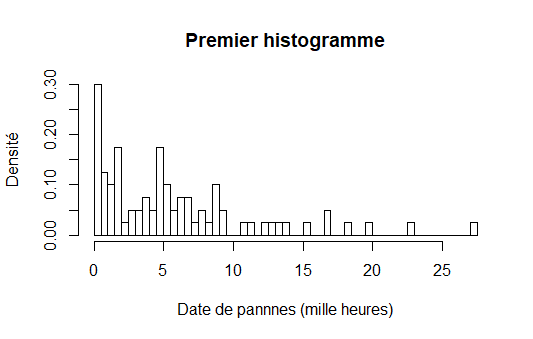
\includegraphics[width=\textwidth]{premier_histo.png}
    \caption{Le premier histogramme de distribution de pannes}
    \label{histo1}
\end{figure}

Les pannes se concentrent autour de 2 sommets, l'un à $[0; 0,5]$ et l'autre à $[4,5; 5]$. Ceci nous fait penser naturellement à un mixage de deux lois.

Comme les valeurs sont positives, et que l'un sommet se situe auprès de zéro et l'autre à une valeur non nulle, nous essayons d'estimer un mixage de loi \emph{Exponentielle} et \emph{Gamma}.

La fonction de densité avec le paramètre $\theta  = \left( {p_1, p_2, \lambda ,\alpha ,\beta } \right)$ :
\begin{align}
    \begin{split}
        \label{fMelExpGam}
        {f_\theta }\left( x \right) & = {p_1}{f_1}\left( x \right) + {p_2}{f_2}\left( x \right) \\
        & = {p_1}\lambda {e^{ - \lambda x}} + {p_2}\frac{{{\beta ^\alpha }}}{{\Gamma \left( \alpha  \right)}}{x^{\alpha  - 1}}{e^{ - \beta x}}
    \end{split}
\end{align}

Où $f_1, f_2$ désignent réspectivement $exp(\lambda)$ et $\Gamma(\alpha, \beta)$; $p_1, p_2 > 0: p_1 + p_2 = 1$.

Nous allons utiliser l'algorithme EM, la méthode la plus efficace pour estimer le MLE de mixage fini.

Soit ${\bf{X}} = \left( {{x_1},...,{x_N}} \right)$ le vecteur des données existants.

Soit la matrice de probabilité d'appartenance $(\zeta_{ki})$ : $\zeta_{ki}$ vaut la probabilité que $x_i$ suive la loi $f_k$.
\begin{equation}
    \label{zeta}
    {\zeta _{ki}} = \frac{{{p_k}{f_k}\left( {{x_i}} \right)}}{{{p_1}{f_1}\left( {{x_i}} \right) + {p_2}{f_2}\left( {{x_i}} \right)}}\forall k = \overline {1,2} \forall i = \overline {1,N}
\end{equation}

La fonction de vraisemblance : 
\begin{equation}
    \label{funlik}
    \ln \Lambda  = \sum\limits_{i = 1}^N {\ln {f_\theta }\left( {{x_i}} \right)}  = \sum\limits_{i = 1}^N {\ln \left( {{p_1}{f_1}\left( {{x_i}} \right) + {p_2}{f_2}\left( {{x_i}} \right)} \right)}
\end{equation}

Nous cherchons à maximiser $\ln \Lambda$ en la dérivant selon $\lambda, \alpha, \beta$.

Pour $\lambda$ :
\begin{align}
    \frac{\partial }{{\partial \lambda }}\ln \Lambda  & = \sum\limits_{i = 1}^N {\frac{{{p_1}{e^{ - \lambda {x_i}}} - {p_1}\lambda {x_i}{e^{ - \lambda {x_i}}}}}{{{p_1}{f_1}\left( {{x_i}} \right) + {p_2}{f_2}\left( {{x_i}} \right)}}} \nonumber \\
    & = \sum\limits_{i = 1}^N {\frac{{{p_1}{f_1}\left( {{x_i}} \right)}}{{{p_1}{f_1}\left( {{x_i}} \right) + {p_2}{f_2}\left( {{x_i}} \right)}}\left( {\frac{1}{\lambda } - {x_i}} \right)} \nonumber  \\
    & = \frac{1}{\lambda }\sum\limits_{i = 1}^N {{\zeta _{1i}}}  - \sum\limits_{i = 1}^N {{\zeta _{1i}}{x_i}}  = 0 \nonumber \\
    \label{lambda}
    \Leftrightarrow \lambda  & = \frac{{\sum\limits_{i = 1}^N {{\zeta _{1i}}} }}{{\sum\limits_{i = 1}^N {{\zeta _{1i}}{x_i}} }}
\end{align}

Pour $\beta$ :
\begin{align}
    \frac{\partial }{{\partial \beta }}\ln \Lambda  & = \sum\limits_{i = 1}^N {\frac{{{p_2}x_i^{\alpha  - 1}}}{{\Gamma \left( \alpha  \right)}}\frac{{\alpha {\beta ^{\alpha  - 1}}{e^{ - \beta {x_i}}} - {\beta ^\alpha }{x_i}{e^{ - \beta {x_i}}}}}{{{p_1}{f_1}\left( {{x_i}} \right) + {p_2}{f_2}\left( {{x_i}} \right)}}} \nonumber \\
    & = \sum\limits_{i = 1}^N {\frac{{{p_2}{f_2}\left( {{x_i}} \right)}}{{{p_1}{f_1}\left( {{x_i}} \right) + {p_2}{f_2}\left( {{x_i}} \right)}}\left( {\frac{\alpha }{\beta } - {x_i}} \right)} \nonumber \nonumber \\
    & = \frac{\alpha }{\beta }\sum\limits_{i = 1}^N {{\zeta _{2i}}}  - \sum\limits_{i = 1}^N {{\zeta _{2i}}{x_i}}  = 0 \nonumber \\
    \label{beta}
    \Leftrightarrow \beta & = \alpha \frac{{\sum\limits_{i = 1}^N {{\zeta _{2i}}} }}{{\sum\limits_{i = 1}^N {{\zeta _{2i}}{x_i}} }}
\end{align}

Pour $\alpha$ : 
\begin{align*}
    \frac{\partial }{{\partial \alpha }}\ln \Lambda  & = \sum\limits_{i = 1}^N {\frac{{{p_2}{e^{ - \beta {x_i}}}}}{{{p_1}{f_1}\left( x \right) + {p_2}{f_2}\left( x \right)}}\left( {\frac{{\beta \left( {\ln \beta  + \ln {x_i}} \right){{\left( {\beta {x_i}} \right)}^{\alpha  - 1}}}}{{\Gamma \left( \alpha  \right)}} - {\beta ^\alpha }{x^{\alpha  - 1}}\frac{{\Psi \left( \alpha  \right)}}{{\Gamma \left( \alpha  \right)}}} \right)} \\
    & = \sum\limits_{i = 1}^N {\frac{{{p_2}{f_2}\left( {{x_i}} \right)}}{{{p_1}{f_1}\left( x \right) + {p_2}{f_2}\left( x \right)}}\left( {\ln \beta  + \ln {x_i} - \Psi \left( \alpha  \right)} \right)} \\
    & = \left( {\sum\limits_{i = 1}^N {{\zeta _{2i}}} } \right)\ln \beta  + \sum\limits_{i = 1}^N {{\zeta _{2i}}\ln {x_i}}  - \Psi \left( \alpha  \right)\left( {\sum\limits_{i = 1}^N {{\zeta _{2i}}} } \right) = 0 \\
    \Leftrightarrow 0 & = \ln \alpha  + \ln \frac{{\sum\limits_{i = 1}^N {{\zeta _{2i}}} }}{{\sum\limits_{i = 1}^N {{\zeta _{2i}}{x_i}} }} + \frac{{\sum\limits_{i = 1}^N {{\zeta _{2i}}\ln {x_i}} }}{{\sum\limits_{i = 1}^N {{\zeta _{2i}}} }} - \Psi \left( \alpha  \right) \text{ (substitué par \eqref{beta})} \\
    \Leftrightarrow 0 & = \ln \alpha  - \Psi \left( \alpha  \right) - c
\end{align*}

Où $c = \ln \left( {\frac{{\sum\limits_{i = 1}^N {{\zeta _{2i}}{x_i}} }}{{\sum\limits_{i = 1}^N {{\zeta _{2i}}} }}} \right) - \frac{{\sum\limits_{i = 1}^N {{\zeta _{2i}}\ln \left( {{x_i}} \right)} }}{{\sum\limits_{i = 1}^N {{\zeta _{2i}}} }}$; $\Psi$ est la fonction digamma.

Selon la méthode de Newton-Rashphon, nous pouvons résoudre $\alpha$ numériquement avec ce formul itératif :
\[{\alpha _{r + 1}} = {\alpha _r} - \frac{{\ln {\alpha _r} + \Psi \left( {{\alpha _r}} \right) - c}}{{\frac{1}{{{\alpha _r}}} - \Psi '\left( {{\alpha _r}} \right)}}\]

\cite{gamma} propose un autre formule convergeant plus vite :
\begin{equation}
    \label{alpha}
    \frac{1}{{{\alpha _{r + 1}}}} = \frac{1}{{{\alpha _r}}} + \frac{{\ln \left( {{\alpha _r}} \right) - \Psi \left( {{\alpha _r}} \right) - c}}{{a_r^2\left( {\frac{1}{{{\alpha _r}}} - \Psi '\left( {{\alpha _r}} \right)} \right)}}
\end{equation}

Avec $\Psi'$ la fonction trigamma. L'itération part avec ${\alpha _0} = \frac{{0.5}}{c}$.

Au final, pour $p_k$:
\begin{equation}
    \label{p}
    {p_k} = \frac{{\sum\limits_{i = 1}^N {{\zeta _{ki}}} }}{N}\forall k = \overline {1,2}
\end{equation}

Etant donné \eqref{zeta}, \eqref{lambda}, \eqref{beta}, \eqref{alpha} et \eqref{p}, nous définissons l'algorithme EM :
\begin{enumerate}
    \item \textbf{Initialisation :} Choisir un $\theta_{vieux}$.
    \item \textbf{Etape E :} Evaluer $(\zeta_{ki})$ sachant $\theta_{vieux}$ en utilisant \eqref{zeta}.
    \item \textbf{Etape M :} Calculer $\theta_{nouveau}$ à l'aide des équations \eqref{lambda}, \eqref{beta}, \eqref{alpha} et \eqref{p}. \\
    \emph{Note :} Pour $\alpha$, l'itération se termine quand $\left| {{\alpha _{r + 1}} - {\alpha _r}} \right| < {\varepsilon_\alpha }$ où $\varepsilon_\alpha$ est un réel positif fixé à l'initialisation.
    \item \textbf{Evaluation :} Si $\left\| {{\theta _{c + 1}} - {\theta _c}} \right\| < {\varepsilon _\theta }$ ($\varepsilon_\theta$ est un réel positif fixé à l'initialisation), l'algorithme s'arrête et $\theta = \theta_{vieux}$. \\ Sinon, reviens à l'étape E avec $\theta_{vieux} \leftarrow \theta_{nouveau}$.
\end{enumerate}

Basé sur le résultat obtenu, nous traçons la fonction de densité $f_\theta$ trouvé (figure \ref{mixage}) et réalisons un test de Kolmogorov-Smirnov qui donne $p-value=0,9663111$ signifiant $96,63\%$ de nous tromper si nous rejetons ce modèle. Nous l'acceptons alors, quoiqu'il ne génère pas 2 sommets comme la remarque initiale. Le code est trouvable à l'annexe \ref{annexe:em_exp_gamma}.

\begin{figure}[!hbt]
    \centering
    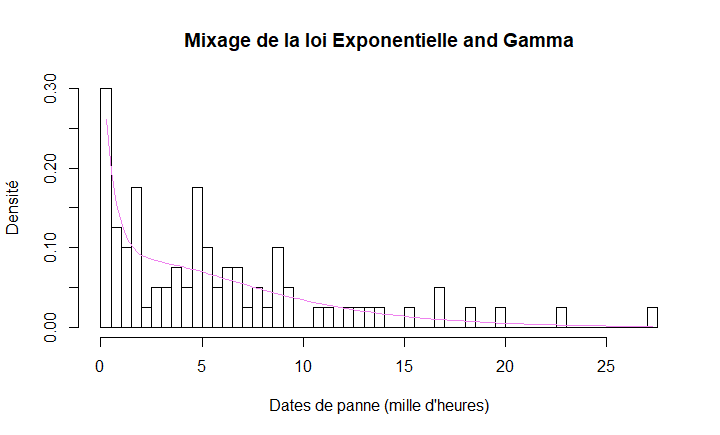
\includegraphics[width=\textwidth]{EM_Exp_Gamma.png}
    \caption{Mixage de la loi Exponentielle et Gamma}
    \label{mixage}
\end{figure}

\subsection{La politique de maintenance basée sur l'âge}


\section{Annexe}
\subsection{L'importation de données de pannes}
\label{annexe:import_pannes}
\lstinputlisting[language=R]{import_failures.R}
\subsection{Le premier histogramme de distribution de pannes}
\label{annexe:premier_histo}
\lstinputlisting[language=R]{premier_histo.R}
\subsection{Estimer le mixage de la loi Exponentielle et Gamma}
\label{annexe:em_exp_gamma}
\lstinputlisting[language=R]{EM_Exp_Gamma.R}

\begin{thebibliography}{9}
    \bibitem{gamma} Minka, Thomas P. (2002). "Estimating a Gamma distribution"

    \url{https://tminka.github.io/papers/minka-gamma.pdf}
\end{thebibliography}
\end{document}